\section{Introduction}
\seclabel{intro}


\newcommand{\xidx}{i}
\newcommand{\yidx}{j}
\newcommand{\xw}[1]{w_{#1}}
\newcommand{\yw}[1]{w'_{#1}}

Dynamic Programming algorithms (DP) build optimal solutions to a problem by combining
together optimal solutions to many overlapping subproblems.  DP
algorithms exploit this overlap to explore otherwise exponential-sized
problem spaces in polynomial time, making them central to many
important applications ranging from logistics to computational
biology. A recent textbook \cite{DurbinEdKr98} on biological sequence analysis, for example,
lists $11$ applications of DP in bioinformatics in its introductory
chapter with many more in chapters that follow.


Dynamic programs are usually described through recurrence relations
that specify how the cells in a DP table must be filled up
using solutions already computed for other cells, but recent research has shown that it is possible
to achieve order-of-magnitude performance improvements over this
standard implementation approach by developing \emph{divide-and-conquer}
 implementation strategies that recursively
partition the problem into smaller subproblems.  These strategies
exhibit better temporal locality, and the partitioning can expose more
optimization opportunities (see, e.g., \cite{IPDPS15/Tithi}). 
Even when compared with tiled implementations optimized by the best polyhedral compilers, 
the divide-and-conquer implementations still show significantly better performance, in some cases
by more than an order of magnitude as illustrated in \figref{performance}. 
\asolar{Have these graphs been published in other papers? If yes, we need to say so and write the previous  par a little differently}
\rch{Those plots appear in \cite{IPDPS15/Tithi}}
Unfortunately, developing such implementations is quite difficult, as will become apparent in \secref{divideConquer}. 
In this paper, we develop a new computer aided approach to formally deriving provably correct divide-and-conquer algorithms
for dynamic programming problems. The approach relies on a new method to formalize the derivation of these algorithms, which
allows an algorithm designer to guide the derivation process through a small number of very high-level tactics. 
Specifically, our paper makes the following contributions:
\begin{enumerate}
  \item We develop a small set of formal tactics that can be used to transform a class of recurrence
  specifications, written in a simple functional language, 
  into equivalent divide-and-conquer programs, that admit parallel cache-local
  implementations, in a principled, systematic manner.
  \item We prove that these tactics are semantics-preserving, assuming some side conditions are met
  at the point when the tactic is applied.
  \item We show that the side conditions can be effectively translated into first-order closed
  formulas, and verified automatically by SMT solvers.
\end{enumerate}



\begin{figure*}
\resizebox{\textwidth}{!}{
\begin{tikzpicture}
	\begin{axis}[
	    title=Parenthesis,
	    ymode=log,
		xlabel=$n$,
		ylabel=Time ({\it s}),
		scaled x ticks=false, %{real:1000}
		log basis y=2, ymajorgrids=true]
	\addplot[color=blue!50!white,ultra thick,mark=*,smooth] table[x=n/Time(s),y=COZ] {data/plot1.dat}
	  [yshift=-8pt] node[pos=0] {CO};
	\addplot[color=red!70!white,ultra thick,mark=*,smooth] table[x=n/Time(s),y=Tiled/Par] {data/plot1.dat}
	  [yshift=-10pt] node[pos=0] {PluTo};
	\end{axis}
\end{tikzpicture}
\begin{tikzpicture}
	\begin{axis}[
	    title=Gap,
	    ymode=log,
		xlabel=$n$,
		scaled x ticks=false, %{real:1000}
		log basis y=2, ymajorgrids=true]
	\addplot[color=blue!50!white,ultra thick,mark=*,smooth] table[x=n/Time(s),y=COZ] {data/plot2.dat}
	  [yshift=-8pt] node[pos=0] {CO};
	\addplot[color=red!70!white,ultra thick,mark=*,smooth] table[x=n/Time(s),y=Tiled/Par] {data/plot2.dat}
	  [yshift=-8pt] node[pos=0] {PoCC};
	\end{axis}
\end{tikzpicture}
\begin{tikzpicture}
	\begin{axis}[
	    title=Floyd-Warshall,
	    ymode=log,
		xlabel=$n$,
		scaled x ticks=false, %{real:1000}
		log basis y=2, ymajorgrids=true]
	\addplot[color=blue!50!white,ultra thick,mark=*,smooth] table[x=n/Time(s),y=COZ] {data/plot3.dat}
	  [yshift=-8pt] node[pos=0] {CO};
	\addplot[color=red!70!white,ultra thick,mark=*,smooth] table[x=n/Time(s),y=Tiled/Par] {data/plot3.dat}
	  [yshift=-8pt] node[pos=0] {PoCC};
	\end{axis}
\end{tikzpicture}
}
\caption{\figlabel{performance}
  Comparison of the the best performance obtained using polyhedral compilers 
  (PluTo\,\cite{HPC10/Pouchet}, PoCC\,\cite{PLDI08/Bondhugula})
  for parallelization, vs. manually crafted recursive divide-and-conquer implementations (CO).}
\end{figure*}

\section{Divide and Conquer DP}
\seclabel{divConquer}
As a motivating example, we consider the Simplified Arbiter problem.
Two processes $x$ and $y$ are scheduled to run $|x|$ and $|y|$ time slots,
respectively. Execution starts at $t=0$, and the length of each time slot is
one time unit. The cost for scheduling the slots $[i..p)$ of $x$ at $t=i+j$
is given by $\xw{ipj}$, and the cost for schedulting the slots $[j..q)$ of $y$
also at $t=i+j$ is given by $\yw{jqi}$.

\begin{figure}
\begin{tabular}{@{\hspace{-1pt}}r@{\hspace{-22pt}}p{3in}}
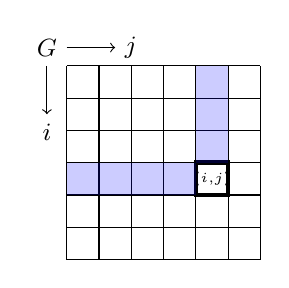
\begin{tikzpicture}[x=4.1mm,y=4.1mm,baseline=(center)]
  \coordinate(center) at (3,3);
  \draw[step=1] (0,0) grid (6,6);
  \draw[ultra thick] (4,2) rectangle +(1,1);
  \node at (4.5,2.5) {\tiny $\scriptscriptstyle\langle i,j\rangle$};
  \fill[blue,opacity=0.2] (0,2) rectangle (4,3);
  \fill[blue,opacity=0.2] (4,3) rectangle (5,6);
  \node[anchor=south east](G) at (0,6) {\small$G$};
  \draw[->] (G.east) -- +(1.5,0) node[anchor=west] {\small $j$};
  \draw[->] (G.south) -- +(0,-1.5) node[anchor=north] {\small $i$};
\end{tikzpicture}
\vspace{10pt}
%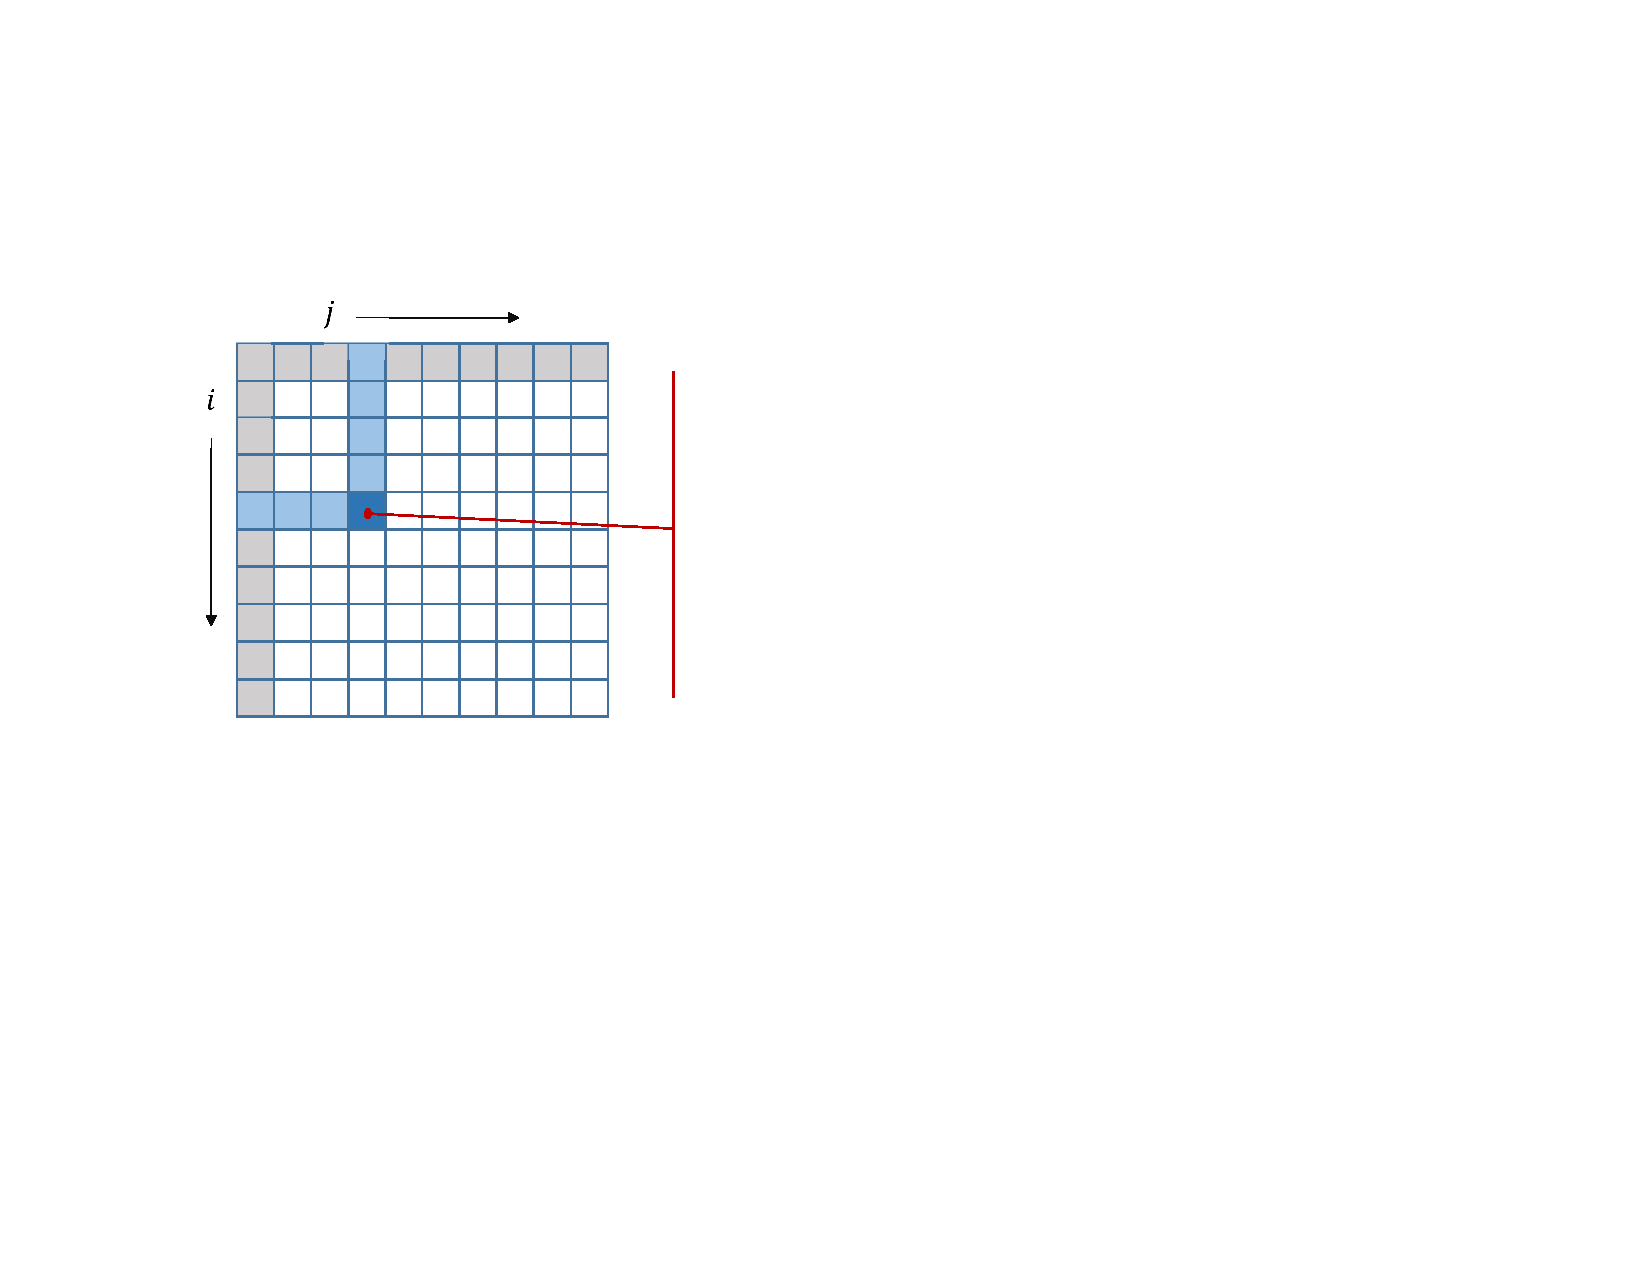
\includegraphics[scale=0.4, bb= 99  445  290 494]{./img/gap1.pdf}
&
\vspace{-50pt}
{\small
\[
\begin{array}{l@{}l}
	G_{ij} &~=~ \\
	&\hspace{-10pt}\begin{cases}
		0                        & i=j=0 \\
		\yw{0j0}                  & i=0, j>0 \\
		\xw{0i0}                 & i>0, j=0 \\
		\begin{array}{@{}l@{\hspace{-1pt}}l@{\hspace{-4pt}}}
		  \min\langle & \underset{0\leq q<j}\min ~ G_{iq} + \yw{qji},  \\
		              & \underset{0\leq p<i}\min ~ G_{pj} + \xw{pij}~\rangle
		\end{array}              & i,j>0
	\end{cases}
\end{array}
\]
}
\end{tabular}
\caption{Recurence equation.}
\figlabel{spec}
\end{figure}


The optimal cost for scheduling the first $i$ slots of $x$ and the first $j$ slots
of $y$ is given by the recurrence in \figref{spec}. When $i$ is zero, it means that
only $y$ has been scheduled, so the cost is $\yw{0j0}$, and similarly when $j$ is zero, 
the cost is $\xw{0i0}$. In the general case, either the schedule ends with time allocated to $x$, 
in which case $x$ was allocated time from some step $p$ to $i$, and the cost is 
$G_{pj} + \xw{pij}$, or the schedule ends with time allocated to $y$, in which case, 
$y$ was allocated time from some step $q$ to $j$, and the cost is $G_{iq} + \yw{qji}$.
In order to determine which is the case, and what is the optimal value of $p$ and $q$, 
the dynamic programming algorithm needs information from all cells above and to the right of $G_{ij}$ as illustrated
in \figref{spec}. Once the algorithm completes the table, one can read the total cost of the entire schedule from $G_{|x||y|}$.

\subsection{Iterative algorithm}

With standard dynamic programming, this recurrence can be computed
with an iterative program by understanding the dependency pattern:
each value $G_{ij}$ is computed from other values $G_{i'j'}$ with lower
indexes, $i'<i$, ~$j'<j$ (see \Cref{intro:arbiter dependency matrix}). 
Therefore, considering $G$ as a two-dimensional
array, it can be filled in a single pass from left to right and from top
to bottom.

\newcommand\FORLINE[1]{\STATE\algorithmicfor~{#1} \algorithmicdo~}

\begin{algorithm}
\renewcommand\arraystretch{1.3}
\begin{algorithmic}
  \STATE $G_{00} := 0$
  \FORLINE{$j=1..|y|$}  $G_{0j} := \yw{0j0}$  
  \FOR{$i=1..|x|$}
    \STATE $G_{i0} := \xw{0i0}$
    \FOR{$j=1..|y|$}
      \STATE $G_{ij} :=
        \begin{array}[t]{@{}l@{~}l} 
          \min\langle & \underset{0\leq q<j}\min ~ G_{iq} + \yw{qji}, \underset{0\leq p<i}\min ~ G_{pj} + \xw{pij}~\rangle \\         
        \end{array}$
    \ENDFOR
  \ENDFOR
\end{algorithmic}
\end{algorithm}

\subsection{Divide and Conquer algorithm}
\newcommand\qbox[1]{\fbox{\scriptsize#1}}
\begin{figure}
\begin{tabular}{p{2in}p{2in}}
$
\renewcommand\arraystretch{2}
\begin{array}{c|c|c|c|}
  \multicolumn{2}{c}{} & \multicolumn{2}{c}{K} \\ \cline{3-4}
  \multicolumn{2}{c}{} & \multicolumn{1}{c}{K_0}  & \multicolumn{1}{c}{K_1}\\ \cline{3-4}
  \multirow{2}{*}{$J$} & J_0 & 1 & 2 \\ \cline{3-4}
    & J_1 & 3 & 4 \\ \cline{3-4}
\end{array}
$
& 
$\begin{array}{l}\qbox1 \rightsquigarrow \qbox2 \\ 
\qbox1 \rightsquigarrow \qbox3 \\ \qbox2\rightsquigarrow \qbox4 \\ \qbox3 \rightsquigarrow \qbox4\end{array}$
\end{tabular}
\caption{\figlabel{quadrants}
  Dividing a two-dimensional array into quadrants; the dependencies are shown on the right.}
\end{figure}

In the divide-and-conquer algorithm, the array $G$ is partitioned into
quadrants as illustrated in \figref{quadrants}, so the same reasoning we applied 
in the iterative case leads us to conclude that the computations of 2 and 3 depend on 1,
and the computation of 4 depends on 2 and 3.

The computation of these quadrants can be \emph{stratified} into the following
four steps:
\begin{algorithmic}[1]
  \STATE Compute \qbox1 (using only input data $w,w'$).
  \STATE Compute \qbox2 using data from \qbox1.
  \STATE Compute \qbox3 using data from \qbox1.
  \STATE Compute \qbox4 using data from \qbox2 and \qbox3.
\end{algorithmic}
Each step depends only on a subset of the steps that came before it, 
as illustrated by \figref{chain}. However, this is not yet a divide-and-conquer algorithm; 
of the four steps, only step \qbox1{} is an instance of the original problem; all the other steps
look somewhat different from the original problem and lack significant locality. With some algebraic manipulation, however, 
it is possible to define each of the four steps above recursively, leading to a true divide-and-conquer algorithm with very high locality 
and significantly improved performance relative to the iterative algorithm.

\newcommand{\range}[1]{\mathcal{D}(#1)}
\newcommand{\real}{\mathcal{R}}

To illustrate how this is done, we first introduce a small amount of notation. First, we use $\range{A,B\ldots}$ as a shorthand
for $(A\times B\times\ldots) \rightarrow \real$. 
As a first step, we will introduce types into the original definition of the algorithm from \figref{spec}. 
\newcommand{\xsub}[1]{subx(#1)}
\newcommand{\ysub}[1]{suby(#1)}

\begin{equation}
\begin{array}{l@{}l}
	G_{i,j,\xw{},\yw{}}:\range{J,K,\range{J,J,K}, \range{K,K,J}} ~=~  \\
	\qquad
	\begin{cases}
		0                        & i=j=0 \\
		w_{0j0}                   & i=0, j>0 \\
		w'_{0i0}                  & i>0, j=0 \\
		\begin{array}{@{}l@{~}l}
		  \min\langle & \underset{q\in[0,j)}\min ~ G_{i,q,\xw{}, \yw{}} + \yw{qji}, \\
		              &\underset{p\in[0,i)}\min ~ G_{pj,\xw{}, \yw{}} + \xw{pij}~\rangle
		\end{array}              & i,j>0
	\end{cases}
\\
%\ysub{i,j,\xw{}, [0,j) }
\end{array}
\end{equation}

The computation of \qbox1{} corresponds to computing $G$ within the sub-domain 
$\range{J_0,K_0,\range{J_0,J_0,K_0}, \range{K_0,K_0,J_0}}$, making it an exact copy of $G$. On the other hand, 
the computation of \qbox2{} has the type  $\range{J_0,K_1,\range{J_0,J_0,K}, \range{K,K,J_0}}$, and the recursive calls
are not confined to \qbox2{}. 

\newcommand{\Ggen}{A}

This can be addressed by generalizing the computation of $G$ in the following way. 
\asolar{I defined $\Ggen$ as a macro. The current name is not very good, but it can be easily changed}


\begin{equation}
\begin{array}{l@{}l}
	\Ggen_{i,j, \psi, \xw{},\yw{}, }:\range{J,K, \range{J,K}, \range{J,J,K}, \range{K,K,J}} ~=~  \\
	\qquad
	\begin{cases}
		0                        & i=j=0 \\
		w_{0j0}                   & i=0, j>0 \\
		w'_{0i0}                  & i>0, j=0 \\
		\begin{array}{@{}l@{~}l}
		  \min\langle & \psi_{ij}, \underset{q\in K\cap[0,j)}\min ~ G_{i,q,\xw{}, \yw{}} + \yw{qji}, \\
		              &\underset{p\in[0,i)}\min ~ G_{pj,\xw{}, \yw{}} + \xw{pij}~\rangle
		\end{array}              & i,j>0
	\end{cases}
\\
\end{array}
\end{equation}

It is easy to see that both $G$ and \qbox1{} can be expressed in terms of $\Ggen$ by making $\psi_{ij}=\infty$, but \qbox2{} can now also be expressed in terms of $\Ggen$ by making $\psi_{ij} =  \underset{q\in K}\min ~ G_{i,q,\xw{}, \yw{}} + \yw{qji}$. Moreover, because the parameters of the calls to $G$ inside $\Ggen$ are now guaranteed to stay within the input range of $\Ggen$, they can be replaced with recursive calls to $\Ggen$ itself. $\Ggen$ can be further generalized so that it can also be used to compute \qbox3{} and \qbox4{}. The sub-computation of $\psi$ can also be transformed into a recursive divide-and-conquer subcomputation, further improving the locality of the resulting algorithm. So through these kind of transformations, it is possible to break the computation of the original $G$ into four subcomputations, each of which is isomorphic to the original, and therefore, each of which can be itself recursively partitioned into four subcomputations, giving us a true divide-and-conquer algorithm. 

As was outlined in \secref{intro}, prior work has shown that the performance results that can be achieved through these transformations can be dramatic. Unfortunately, the line of reasoning that was followed in the preceding section can get quite complicated for most dynamic programming algorithms, and producing a correct divide-and-conquer algorithm for a given dynamic programming problem is considered quite difficult even by the researchers who originally pioneered this technique. In the next section, we formalize our approach for deriving divide-and-conquer DP algorithms and describe our computer aided approach for generating provably correct divide-and-conquer DP.


\subsection{old stuff}


 $G_{\,(i : J_0)\,(j : K_0)}$; \ie{} it is the
 same as that of G, but restricted to $J_0$ and $K_0$. Similarly, the computation of \qbox2{} corresponds to $G_{\,(i : J_0)\,(j : K_1)}$; 
note that in this case, however, the range of $q$ in $\ysub{}$ will not be limited to $K_1$, but instead has to range over all of $K$. 
In order to make recursive sub-problems, the computation of \qbox2 can be broken down in the following way: 
\begin{equation}
\begin{array}{l@{}l}
	G_{\,(i : J_0)\,(j : K_1)} ~=~  \\
	\qquad
	\begin{cases}
		0                        & i=j=0 \\
		w_{0j0}                   & i=0, j>0 \\
		w'_{0i0}                  & i>0, j=0 \\
		\begin{array}{@{}l@{~}l}
		  \min\langle & \ysub{i,j,K_0 }, \ysub{i,j,K_1 \cap [0,j) }, \\
		              &\xsub{i,j,[0,i)}~\rangle
		\end{array}              & i,j>0
	\end{cases}
\\
\end{array}
\end{equation}

\begin{figure}
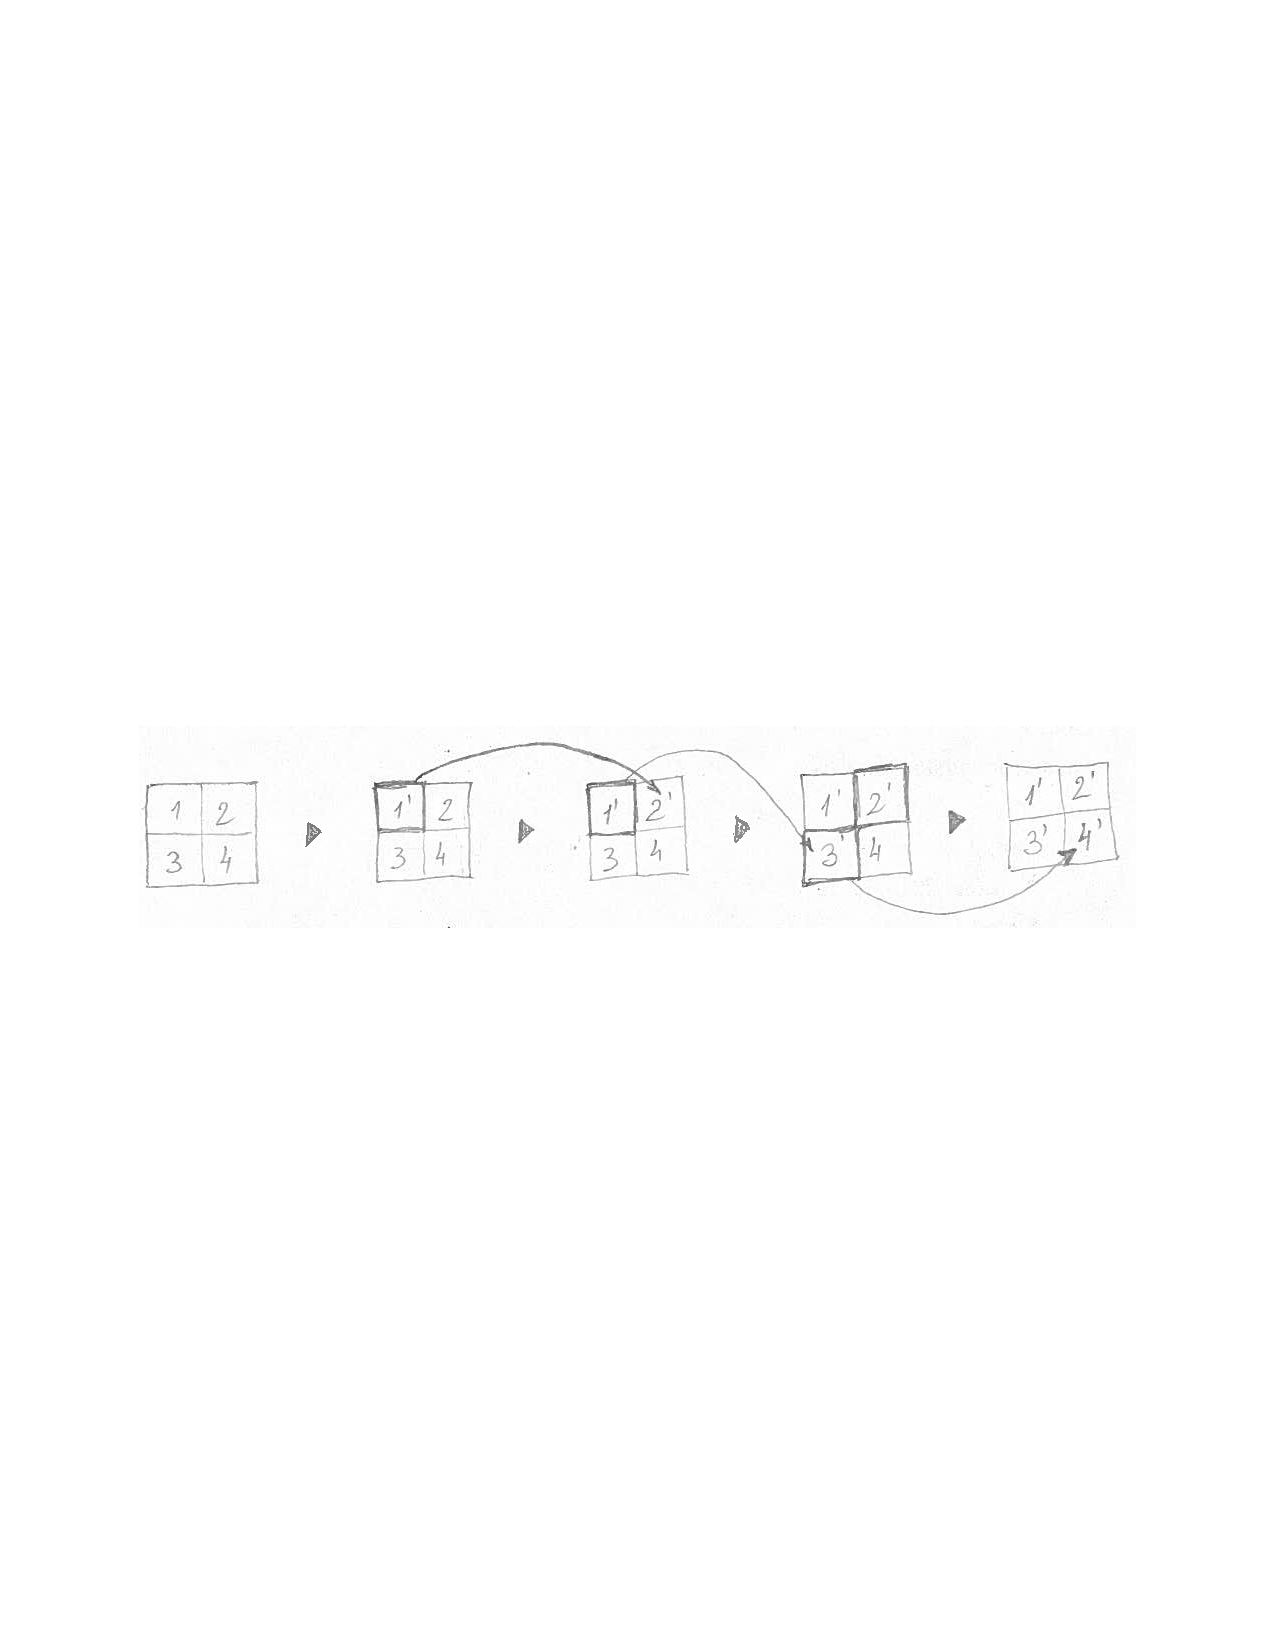
\includegraphics[width=.47\textwidth]{img/gap-stratify1}
\caption[caption]{\figlabel{chain}
  Stratified computation for Simplified Gap. \\[.2em]
  Thick borders indicate the region that is read at each step.}
\end{figure}

At this point it can be noticed that step 1 is equivalent to the original
algorithm when given as input the prefixes of $x$ and $y$ whose length correspond to the
height and width of \qbox1.

With the other three steps, however, things are not so simple:
each of them is required to process some data in addition to the input.
For example, step 2 is required to read values from \qbox1, due to the expression
$G_{iq}$ (where $\scriptstyle 0\leq q<j$).
In order to reason more formally, we define $J$ and $K$ the index sets of the rows
and columns, respectively; $J_0$, $J_1$ for the top and bottom row indexes, respectively;
and $K_0$, $K_1$ for the left and right column indexes (\Cref{intro:slice G}).
The specifications for step 2 then take the following form:

\begin{equation}\LeftEqNo
\renewcommand\arraystretch{1.5}
\begin{array}{l@{}l}
	G_{\,(i : J_0)\,(j : K_1)} ~=~  \\
	\qquad
	\begin{cases}
		0                        & i=j=0 \\
		w'_{0j0}                 & i=0, j>0 \\
		w_{0i0}                  & i>0, j=0 \\
		\begin{array}{@{}l@{~}l}
		  \min\langle & \underset{0\leq (q:K) <j}\min ~ G_{iq} + w'_{qji}, \\
		              & \underset{0\leq (p:J_0) <i}\min ~ G_{pj} + w_{pij}~\rangle
		\end{array}              & i,j>0
	\end{cases}
\end{array}
\end{equation}

\medskip
Type annotations have been placed on $i$, $j$, $p$, and $q$ to define the regions
over which they range. $i:J_0, j:K_1$ means that the element $G_{ij}$
is always in \qbox2. Similarly, $G_{pj}$ is also in \qbox2. $G_{iq}$ is either in
\qbox1 or in \qbox2.


To address the situation, the algorithm designer would like to separate the parts
of the computation that read from \qbox1 from the parts that read from \qbox2.
This can be achieved here by splitting the $\min_{0\leq(q:K)<j}$ into two
ranges, according to the region in which $G_{iq}$ resides.

\begin{equation}\LeftEqNo
\renewcommand\arraystretch{1.5}
\begin{array}{l@{}l}
	G_{\,(i : J_0)\,(j : K_1)} ~=~  \\
	\qquad
	\begin{cases}
		0                        & i=j=0 \\
		w'_{0j0}                 & i=0, j>0 \\
		w_{0i0}                  & i>0, j=0 \\
		\begin{array}{@{}l@{~}l}
		  \min\langle & \underset{(q:K_0)}\min ~ G_{iq} + w'_{qji}, \\
		              & \underset{(q:K_1) <j}\min ~ G_{iq} + w'_{qji}, \\
		              & \underset{0\leq (p:J_0) <i}\min ~ G_{pj} + w_{pij}~\rangle
		\end{array}              & i,j>0
	\end{cases}
\end{array}
\end{equation}

\medskip
The path becomes clear: compute $\min_{(q:K_0)} ~ G_{iq} + w_{qj}$ first, for all $i$, $j$
in \qbox2. Then use the results to compute $G_{ij}$.

\begin{equation}\LeftEqNo
\renewcommand\arraystretch{1.5}
\begin{array}{l@{}l}
	G_{\,(i : J_0)\,(j : K_1)} ~=~  \\
	\qquad
	\textrm{let}~\psi_{ij} = \underset{(q::K_0)}\min ~ G_{iq} + w'_{qji} \\
	\qquad\textrm{in} \\
	\qquad
	\begin{cases}
		0                        & i=j=0 \\
		w'_{0j0}                 & i=0, j>0 \\
		w_{0i0}                  & i>0, j=0 \\
		\begin{array}{@{}l@{~}l}
		  \min\langle & \psi_{ij}, \\
		              & \underset{(q:K_1) <j}\min ~ G_{iq} + w'_{qji}, \\
		              & \underset{0\leq (p:J_0) <i}\min ~ G_{pj} + w_{pij}~\rangle
		\end{array}              & i,j>0
	\end{cases}
\end{array}
\label{intro:let in 2}
\end{equation}

\medskip
The second part in \eqref{intro:let in 2} starts to look similar to \eqref{intro:arbiter spec}:
in particular, the types of $p$ and $q$ are the same as those of $i$ and $j$.
In fact, if we set $\psi_{ij}=\infty$, we get \eqref{intro:arbiter spec} as a special case,
only with $J_0$ and $K_1$ instead of $J$ and $K$.
It therefore makes sense to write a version that generalizes both.

\begin{equation}\LeftEqNo
\renewcommand\arraystretch{1.5}
\begin{array}{l}
	A^{^{JK}}_{\,\psi ij} ~=~  \\
	\qquad
	\begin{cases}
		0                        & i=j=0 \\
		w'_{0j0}                 & i=0, j>0 \\
		w_{0i0}                  & i>0, j=0 \\
		\begin{array}{@{}l@{~}l}
		  \min\langle & \psi_{ij}, \\
		              & \underset{(q:K)<j}\min ~ A^{^{JK}}_{\psi iq} + w'_{qji}, \\
		              & \underset{(p:J)<i}\min ~ A^{^{JK}}_{\psi pj} + w_{pij}~\rangle
		\end{array}              & i,j>0
	\end{cases}
\end{array}
\label{intro:arbiter phase A}
\end{equation}

\medskip
And we can now rewrite \eqref{intro:arbiter spec} and \eqref{intro:let in 2} as
%
\begin{equation}
	G_{ij} ~=~ A^{^{JK}}_{\,(\infty^{J\times K})\,(i:J)\,(j:K)}
\end{equation}
%
\begin{equation}
\renewcommand\arraystretch{1.3}
\begin{array}{l@{}l}
	G_{\,(i : J_0)\,(j : K_1)} ~=~ 
	& \textrm{let}~\psi_{ij} = \underset{(q:K_0)}\min ~ G_{iq} + w_{qj} \\
	& \textrm{in}~A^{^{J_0K_1}}_{\,\psi ij}
\end{array}	
\label{intro:let in 2 using A}
\end{equation}

\newcommand\otherwise{\textrm{\small otherwise}}

\medskip
It takes a bit more insight to notice that \eqref{intro:let in 2 using A} can be further
generalized into:
%
\begin{equation}\LeftEqNo
\renewcommand\arraystretch{1.5}
\begin{array}{l@{}l}
	A^{^{JK}}_{\,\psi\,(i : J_0)\,(j : K_1)} ~=~ \\
	\qquad
	\textrm{let}~\psi'_{ij} = \begin{cases}
	  \begin{array}{@{}l@{}l@{}}\min\langle & \psi_{ij}, \\ & \!\underset{(q:K_0)}\min ~ A^{^{J_0K_0}}_{\,\psi iq} + w'_{qji}\rangle\end{array} & \langle i,j\rangle\mbox{ in }\qbox2 \\
	  \psi_{ij} & \otherwise
	\end{cases} \\
	\qquad\textrm{in}~
	A^{^{J_0K_1}}_{\,\psi' ij}
\end{array}
\label{intro:let in A 2}
\end{equation}

That is the core of the divide and conquer method: representing the output as a combination
of solutions to sub-problems, yielding an algorithm that is essentially
a recursive routine, or a set of mutually recursive routines. 
Once all the pieces fit together, it is possible to cut the space into arbitrarily small pieces,
that fit nicely in each core's local cache. This greately increases performance, as demonstrated
by~\citneeded{perhaps include a table with exact figures}. 
\todo{Find a way to make this statement earlier}

\medskip
We can apply similar treatment to \qbox3 and \qbox4:
%
\begin{equation}\LeftEqNo
\renewcommand\arraystretch{1.5}
\begin{array}{l@{}l}
	A^{^{JK}}_{\,\psi\,(i : J_1)\,(j : K_0)} ~=~ \\
	\qquad
	\textrm{let}~\psi'_{ij} = \begin{cases} 
	  \begin{array}{@{}l@{}l@{}}\min\langle & \psi_{ij}, \\ & \!\underset{(p:J_0)}\min ~ A^{^{J_0K_0}}_{\,\psi pj} + w_{pij}\rangle \end{array} & \langle i,j\rangle\mbox{ in }\qbox3 \\
	  \psi_{ij} & \otherwise \\
	\end{cases} \\
	\qquad\textrm{in}~
	A^{^{J_1K_0}}_{\,\psi' ij}
\end{array}
\label{intro:let in A 3}
\end{equation}

\begin{equation}\LeftEqNo
\renewcommand\arraystretch{1.5}
\begin{array}{l@{}l}
	A^{^{JK}}_{\,\psi\,(i : J_1)\,(j : K_1)} ~=~ \\
	\qquad
	\textrm{let}~\psi'_{ij} = \begin{cases} 
	  \begin{array}{@{}l@{}l@{}}\min\langle & \psi_{ij}, \\
         & \!\underset{(q:K_0)}\min ~ A^{^{J_1K_0}}_{\,\psi iq} + w'_{qji}\rangle \\
         & \!\underset{(p:J_0)}\min ~ A^{^{J_0K_1}}_{\,\psi pj} + w_{pij}\rangle \end{array} & \langle i,j\rangle\mbox{ in }\qbox4 \\
	  \psi_{ij} & \otherwise \\
	\end{cases} \\
	\qquad\textrm{in}~
	A^{^{J_1K_0}}_{\,\psi' ij}
\end{array}
\label{intro:let in A 4}
\end{equation}

Evidently there are some common sub-expressions. Defining
\begin{equation}
\renewcommand\arraystretch{1.3}
\begin{array}{l@{}l@{}l}
	B^{^{JK_0K_1}}_{\,\psi\,(i : J)\,(j : K_1)} ~=~ &
	  \min\langle & \psi_{ij}, \\ 
	&  & \!\underset{(q:K_0)}\min ~ \psi_{iq} + w'_{qji}\rangle \\[.8em]
	C^{^{J_0J_1K}}_{\,\psi\,(i : J_1)\,(j : K)} ~=~ &
	  \min\langle & \psi_{ij}, \\ 
	&  & \!\underset{(p:J_0)}\min ~ \psi_{pj} + w_{pij}\rangle 
\end{array}
\label{intro:spec of B,C}
\end{equation}

We can write \eqref{intro:let in A 2}, \eqref{intro:let in A 3}, \eqref{intro:let in A 4} as ---

\newcommand\qqquad{\qquad\qquad}

\begin{equation}\LeftEqNo
\renewcommand\arraystretch{1.5}
\begin{array}{@{}l@{}l}
    \lspan2{
	A^{^{JK}}_{\,\psi\,(i : J_0)\,(j : K_1)} ~=~ } \\
	\qqquad
	\textrm{let}~ & \psi'_{ij} = \begin{cases}
	  A^{^{J_0K_0}}_{\psi ij} & \langle i,j\rangle\mbox{ in }\qbox1 \\
	  \psi_{ij} & \otherwise
	\end{cases} \\[1.2em]
	& \psi''_{ij} = \begin{cases}
	  B^{^{J_0K_0K_1}}_{\psi' ij} & \langle i,j\rangle\mbox{ in }\qbox2 \\
	  \psi'_{ij} & \otherwise
	\end{cases} \\
	\lspan2{
	\qqquad\textrm{in}~
	A^{^{J_0K_1}}_{\,\psi'' ij} }
\end{array}
\label{intro:let in A 2 using B}
\end{equation}

\begin{equation}\LeftEqNo
\renewcommand\arraystretch{1.5}
\begin{array}{@{}l@{}l}
    \lspan2{
	A^{^{JK}}_{\,\psi\,(i : J_1)\,(j : K_0)} ~=~ } \\
	\qqquad
	\textrm{let}~ & \psi'_{ij} = \begin{cases}
	  A^{^{J_0K_0}}_{\psi ij} & \langle i,j\rangle\mbox{ in }\qbox1 \\
	  \psi_{ij} & \otherwise
	\end{cases} \\[1.2em]
	& \psi''_{ij} = \begin{cases}
	  C^{^{J_0J_1K_0}}_{\psi ij} & \langle i,j\rangle\mbox{ in }\qbox3 \\
	  \psi_{ij} & \otherwise
	\end{cases} \\
	\lspan2{
	\qqquad\textrm{in}~
	A^{^{J_1K_0}}_{\,\psi' ij} }
\end{array}
\label{intro:let in A 3 using C}
\end{equation}

\begin{equation}\LeftEqNo
\renewcommand\arraystretch{1.5}
\begin{array}{l@{}l}
	\lspan2{A^{^{JK}}_{\,\psi\,(i : J_1)\,(j : K_1)} ~=~} \\
	\qquad
	\textrm{let}~ & \psi'_{ij} = \begin{cases}
	  A^{^{J_0K_1}}_{\psi ij} & \langle i,j\rangle\mbox{ in }\qbox2 \\
	  A^{^{J_1K_0}}_{\psi ij} & \langle i,j\rangle\mbox{ in }\qbox3 \\
	  \psi_{ij} & \otherwise
	\end{cases} \\[1.8em]
	& \psi''_{ij} = \begin{cases}
	  B^{^{J_1K_0K_1}}_{\psi' ij} & \langle i,j\rangle\mbox{ in }\qbox4 \\
	  \psi'_{ij} & \otherwise
	\end{cases} \\[1.2em]
	& \psi'''_{ij} = \begin{cases}
	  C^{^{J_0J_1K_1}}_{\psi'' ij} & \langle i,j\rangle\mbox{ in }\qbox4 \\
	  \psi''_{ij} & \otherwise
	\end{cases} \\
	\lspan2{
	\qquad\textrm{in}~A^{^{J_1K_0}}_{\,\psi''' ij}
	}
\end{array}
\label{intro:let in A 4 using B,C}
\end{equation}

\begin{figure*}
\begin{center}
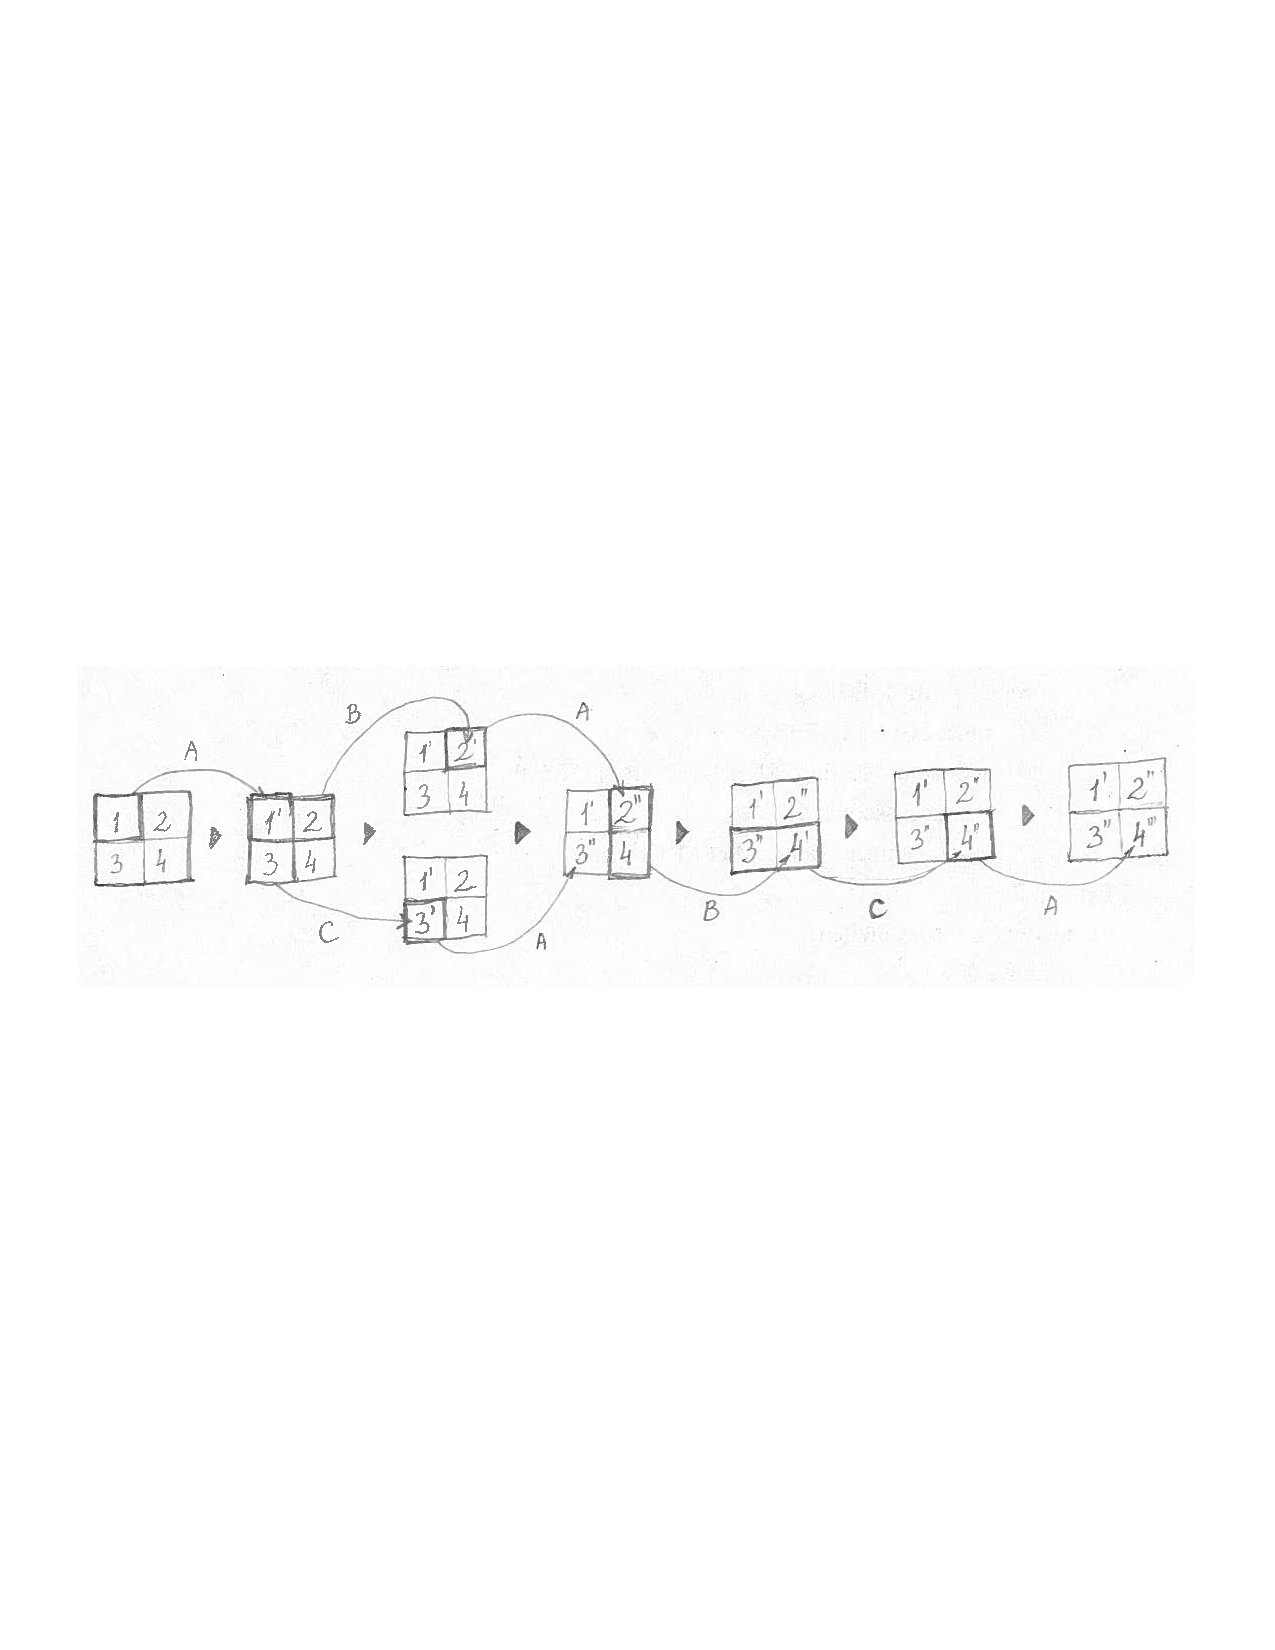
\includegraphics[width=.9\textwidth]{img/gap-stratify-A}
\end{center}
\caption{\label{intro:arbiter stratify A chain}}
\end{figure*}

This leads to the further stratified version shown in \Cref{intro:arbiter stratify A chain}.
The phases
$B$ and $C$ \eqref{intro:spec of B,C} are two more sub-problems that have to be addressed using the same slicing technique.
At first, it may seem that we have completed one task but created two; 
fortunately, $B$ and $C$ are much simpler instances\todo{for once, they are not recursive}
and are quite easy to develop.\todo{show this? Forget about this paragraph??}



\begin{center}$\vdots$
\end{center}


\subsection{Main Contributions}

\begin{enumerate}
  \item We develop a small set of formal tactics that can be used to transform a class of recurrence
  specifications, written in a simple functional language, 
  into equivalent divide-and-conquer programs, that admit parallel cache-local
  implementations, in a principled, systematic manner.
  \item We prove that these tactics are semantics-preserving, assuming some side conditions are met
  at the point when the tactic is applied.
  \item We show that the side conditions can be effectively translated into first-order closed
  formulas, and verified automatically by SMT solvers.
\end{enumerate}

